\chapter{Huấn luyện, thử nghiệm và đánh giá}

Chương này sẽ trình bày chi tiết các kịch bản thử nghiệm để đánh giá hiệu quả của giải pháp co/dãn đa cấp độ chủ động được đề xuất trong chương 3, hệ thống triển khai, đánh giá và theo dõi được nêu rõ tại chương 4. Kết quả thử nghiệm sẽ được đánh giá, phân tích và so sánh nhằm đưa ra kết luận về hiệu năng và hiệu suất của giải pháp hệ thống được để xuất.

\section{Yêu cầu của hệ thống}

Đầu tiên, ta liệt kê lại các tiêu chí yêu cầu của hệ thống đã đề ra làm cơ sở để triển khai các kịch bản thử nghiệm và đánh giá, phân tích sau này.

\begin{itemize}
    \item Cân bằng giữa việc mở rộng và thu hẹp: Đảm bảo không mở rộng quá mức khi hệ thống có chịu được tải, do môi trường triển khai trên hệ thống điện đoán đám mây, bất kỳ tài nguyên không hợp lý nào đều sẽ gây ra lãng phí. Không thu hẹp quá nhiều khiến hệ thống thiếu tài nguyên xử lý, gây ảnh hưởng nghiêm trọng đến trải nghiệm người dùng.
    \item Hiệu năng ổn định: Hệ thống hoạt động ổn định, xuyên suốt.
    \item Tự động cấu hình lại tài nguyên: Hệ thống cần có khả năng tự động cấu hình lại các tài nguyên như máy chủ ảo hoặc container mà không cần sự can thiệp thủ công.
    \item Giám sát hiệu suất: Hệ thống phải có khả năng theo dõi liên tục các chỉ số như \gls{cpu}, bộ nhớ, băng thông mạng và độ trễ.
    \item Hệ thống có khả năng co/dãn các supervisor.
\end{itemize}

\paragraph{Cấu hình của các supervisor xử lý dữ liệu}

\begin{itemize}
    \item Mỗi supervisor có 550 Mb RAM và 1 core \gls{cpu} tương ứng với 1 worker port: 6700.
    \item Số lượng supervisor tối đa là 5 và tối thiểu là 2.
\end{itemize}

\paragraph{Các lưu ý về quá trình đánh giá}

Nhằm đơn giản hóa việc đánh giá, đồ thị tỷ lệ sử dụng bộ nhớ được bổ sung thêm 3 đường tham chiếu, tương ứng từ lớn đến nhỏ là 90\%, 60\% và 20\%. Tại mức tỷ lệ sử dụng bộ nhớ

\begin{itemize}
    \item 90\%: Supervisor đang sử dụng quá nhiều bộ nhớ, khả năng cao trong tương lai sẽ tiếp tục tăng và gây quá tải bộ nhớ làm tăng độ trễ của hệ thống.
    \item 60\%: Supervisor đang sử dụng bộ nhớ ở mức lý tưởng.
    \item 20\%: Supervisor đang gây lãng phí tài nguyên do mức tỷ lệ sử dụng bộ nhớ này tương đương với tiến trình hệ thống supervisor sử dụng, có nghĩa đóng góp của supervisor là không có hoặc không đáng kể.
\end{itemize}

Tại đồ thị số lượng tin gửi đi của spout, đường đồ thị thường có dạng tăng tuyến tính từ 0 đến một ngưỡng nào đó, lý do là bởi Storm UI thu thập dữ liệu theo cửa sổ thời gian mà cụ thể ở đây là 10 phút, vì vậy các đường tăng có dạng tuyến tính có thể được hiểu rằng spout đang truyền tin với tốc độ không đổi.

Các dạng chỉ số mang tính tích lũy như số gói tin truyền đi, phát đi của spout hoặc bolt đều được chuẩn hóa từ dạng cửa sổ 550 giây (10 phút) về cửa sổ 30 giây để tăng tính trực quan do dữ liệu nguyên bản lớn khiến cho việc so sánh gây ra khó khăn. Tuy nhiên, cũng do dữ liệu bị chuẩn hóa nên sẽ gây ra hao hụt, từ đó thể hiện sẽ không thể chính xác tuyệt đối mà chỉ mang tính tương đối gần đúng.

Độ trễ được tính theo đơn vị ms (milli giây) với một luồng dữ liệu tối đa sẽ đi qua 1 spout và 3 bolt, từ đó suy ra trễ trung bình cần không được vượt quá 250 ms đối với mỗi thành phần sẽ đảm bảo hệ thống không bị quá tải khi tổng thời gian xử lý dữ liệu dưới ngưỡng 1 giây.

\section{Thử nghiệm}

\paragraph{Kịch bản thử nghiệm}

Dữ liệu được gửi đến \gls{mqtt} sẽ có các cấu hình được liệt kê tại bảng \ref{tab:mqtt-building-publishers}.

% Please add the following required packages to your document preamble:
% \usepackage{graphicx}
\begin{table}[]
    \centering
    \resizebox{\textwidth}{!}{%
        \begin{tabular}{|l|l|}
            \hline
            Giai đoạn                            & Dữ liệu các tòa nhà đang gửi \\ \hline
            Gửi dữ liệu các tòa nhà 1, 2         & 1, 2                         \\ \hline
            Gửi thêm dữ liệu các tòa nhà 3, 6    & 1, 2, 3, 6                   \\ \hline
            Gửi thêm dữ liệu các tòa nhà 4, 5    & 1, 2, 3, 4, 5, 6             \\ \hline
            Dừng gửi dữ liệu các tòa nhà 1, 6    & 2, 3, 4, 5                   \\ \hline
            Dừng gửi dữ liệu các tòa nhà 2, 4    & 3, 5                         \\ \hline
            Gửi thêm dữ liệu tòa nhà 6           & 3, 5, 6                      \\ \hline
            Dừng gửi dữ liệu toàn bộ các tòa nhà & Không                        \\ \hline
        \end{tabular}%
    }
    \caption{Dữ liệu gửi từ MQTT publisher}
    \label{tab:mqtt-building-publishers}
\end{table}

\subsection{Kết quả  thử nghiệm học tăng cường Q}

\begin{figure}[htbp]
    \centering
    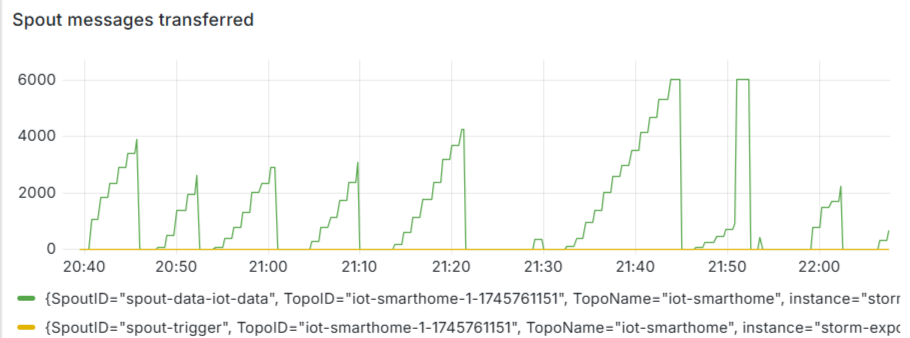
\includegraphics[width=\textwidth]{evaluation-01-messages-transferred.png}
    \caption{Học tăng cường Q - số gói tin gửi đi của các spout}
    \label{fig:evaluate-q-spout-messages-transferred}
\end{figure}

\begin{figure}[htbp]
    \centering
    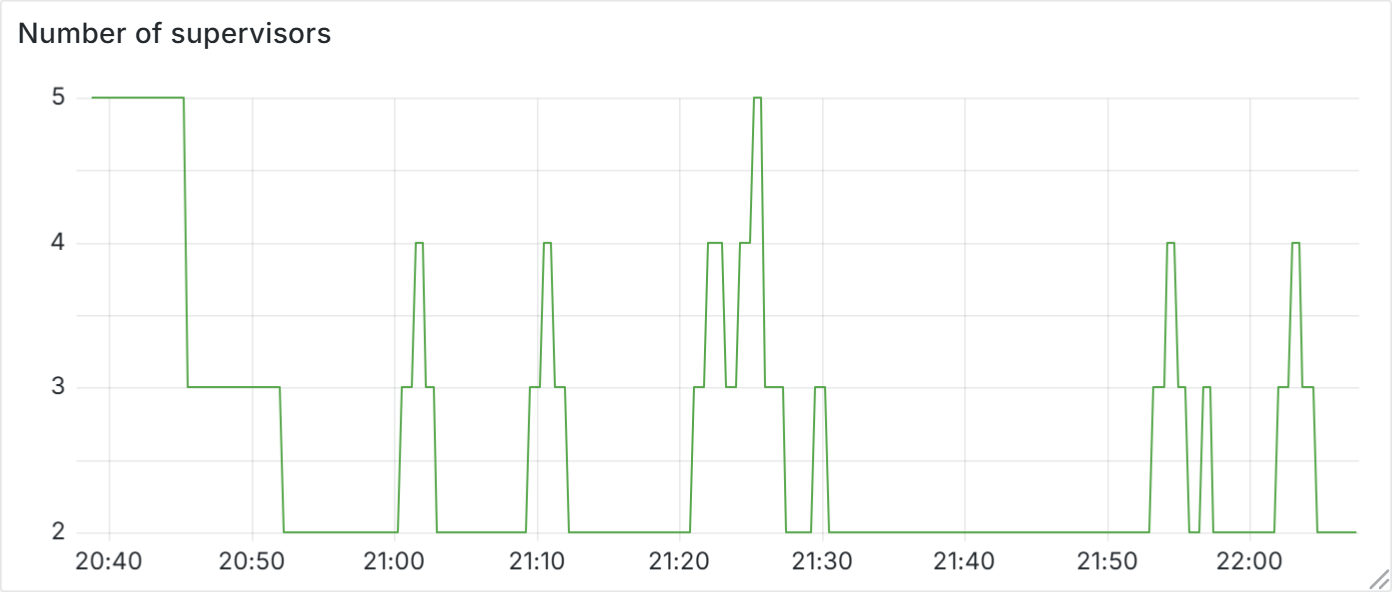
\includegraphics[width=\textwidth]{evaluation-01-number-of-supervisors.png}
    \caption{Học tăng cường Q - số supervisor}
    \label{fig:evaluate-q-supervisors}
\end{figure}

Có thể nhận thấy, hệ thống đã thể hiện khả năng co/dãn số lượng các supervisor khá ổn. Trong hình \ref{fig:evaluate-q-spout-messages-transferred} và hình \ref{fig:evaluate-q-supervisors} tại các thời điểm 21:00, 21:10, 21:20, 21:53, 22:00, khi số lượng gói tin do spout gửi tăng cao, hệ thống đã tiến hành triển khai tăng thêm số lượng supervisor. Tuy nhiên hệ thống vẫn chưa hoạt động đủ tốt trong khoảng thời gian từ 21:30 đến 21:50 khi số lượng gói tin tăng cao lên đến đỉnh điểm nhưng hệ thống không hề có phản ứng tăng số lượng supervisor.

\begin{figure}[htbp]
    \centering
    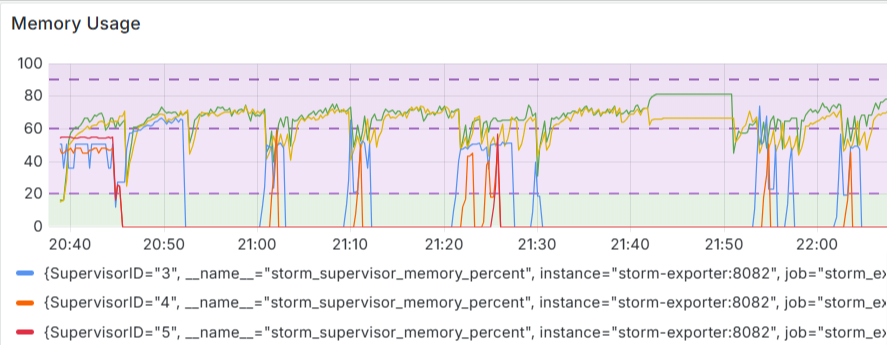
\includegraphics[width=\textwidth]{evaluation-01-memory-percent.png}
    \caption{Theo dõi tỷ lệ sử dụng bộ nhớ của các supervisor trong giai đoạn đánh giá}
    \label{fig:evaluate-d-memory-usage}
\end{figure}

Từ hình \ref{fig:evaluate-d-memory-usage}, có thể thấy hệ thống có thể tối ưu tỷ lệ sử dụng bộ nhớ khá tốt khi các supervisor đều có tỷ lệ sử dụng bộ nhớ quanh khoảng lý tưởng được định ra là 60\%. Tương ứng với khoảng thời gian 21:30 đến 21:50 như bên trên đã nói, ta có thể thấy tuy chỉ có 2 supervisor với số lượng gói tin gửi tăng cao nhưng trên thực tế, tỷ lệ sử dụng bộ nhớ của từng supervisor tuy không nằm gần ngưỡng lý tưởng nhưng vẫn ở trong khoảng cho phép. Khi ở trong khoảng này, giá trị phạt do tỷ lệ sử dụng bộ nhớ bị lệch khỏi tỷ lệ lý tưởng không quá lớn và được bù đắp bởi mức thưởng ổn định khi không thay đổi số lượng supervisor.

\begin{figure}[htbp]
    \centering
    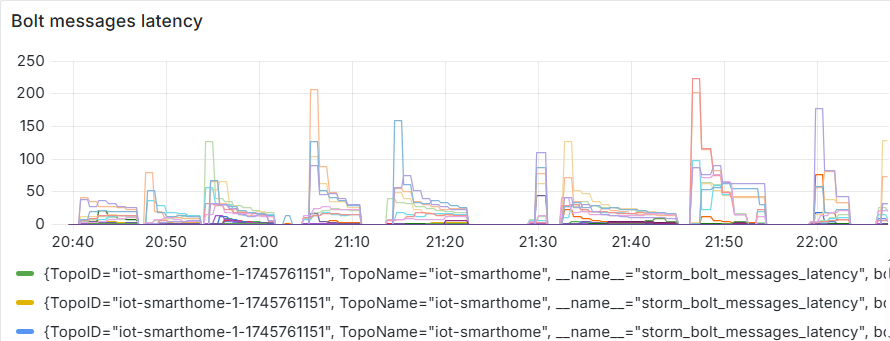
\includegraphics[width=\textwidth]{evaluation-01-bolt-messages-latency.png}
    \caption{Học tăng cường Q - Độ trễ gói tin của các bolt}
\end{figure}

Có thể nhận thấy, hệ thống đã có thể co/dãn số lượng supervisor để đáp ứng nhu cầu tải của hệ thống, khi độ trễ của gói tin của các bolt tăng cao, hệ thống đã đáp ứng bằng cách tăng số lượng supervisor lên để giảm tải khối lượng công việc cần xử lý của từng supervisor. Ví dụ, tại các thời điểm 20:56 và 21:06, độ trễ của các bolt tăng cao đột biến thì tại các thời điểm 21:00 và 21:09 hệ thống đã tăng liên tục từ 2 supervisor lên 4 supervisor để giảm tải giữa các supervisor.

\subsection{Kết quả  thử nghiệm học tăng cường Q sâu}

\begin{figure}
    \centering
    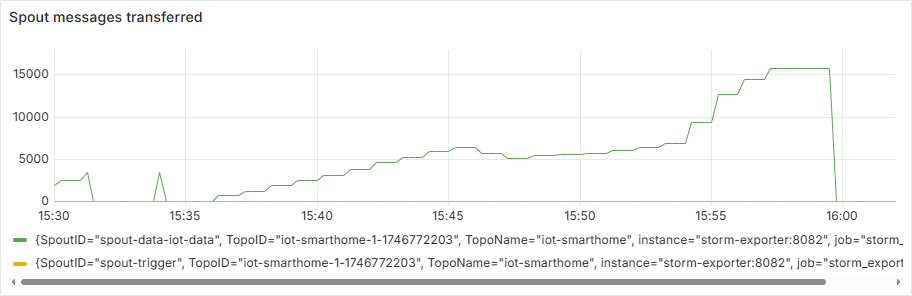
\includegraphics[width=\textwidth]{dq-scale/spout-messages-transferred-01.png}
    \caption{Học tăng cường Q sâu - số gói tin gửi đi của các spout}
    \label{fig:evaluate-dq-spout-messages-transferred}
\end{figure}

\begin{figure}
    \centering
    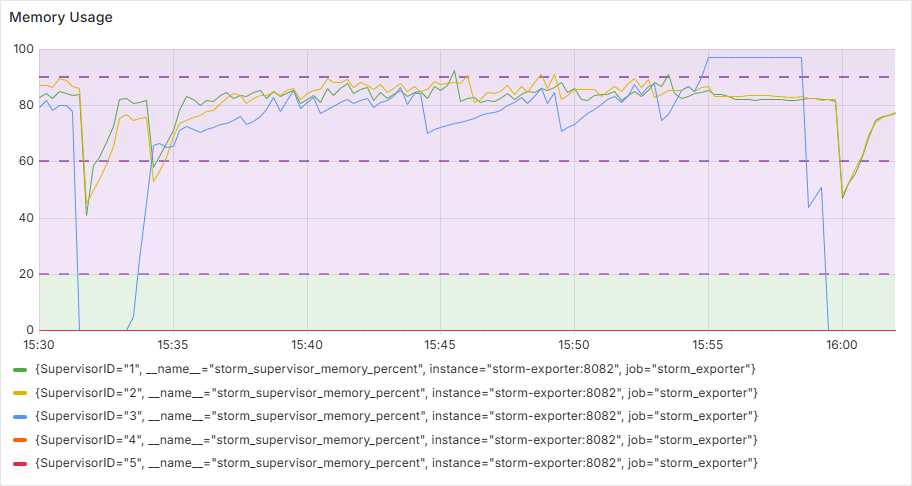
\includegraphics[width=\textwidth]{dq-scale/supervisors-memory-usage-01.png}
    \caption{Học tăng cường Q sâu - tỷ lệ sử dụng bộ nhớ của các supervisor}
    \label{fig:evaluate-dq-memory-usage}
\end{figure}

Tương tự như với học tăng cường Q, ta có thể nhận định rằng hệ thống đã có thể co/dãn supervisor dựa trên tải thực tế của hệ thống. Trong hình \ref{fig:evaluate-dq-spout-messages-transferred} tại thời điểm sau 15:35 số gói tin bắt đầu tăng, số lượng supervisor cũng theo đó tăng theo. Tại thời điểm 16:00, số gói tin giảm đột ngột về giá trị 0, số lượng supervisor cũng theo đó giảm đi.

% Tương tự như với học tăng cường Q, ta có thể nhận định rằng hệ thống đã có thể co/dãn supervisor dựa trên tải thực tế của hệ thống. Trong hình \ref{fig:evaluate-dq-spout-messages-transferred} tại các thời điểm 19:29 và 19:45 số lượng các gói tin gửi đi giảm mạnh, do đó số lượng supervisor cũng bị giảm đi tương ứng, tại thời điểm gần 19:35 khi số lượng gói tin bắt đầu tăng trở lại, thì số supervisor cũng được điều chỉnh theo. Lý do mà hệ thống học tăng cường sâu Q luôn duy trì số lượng supervisor ở mức cao là tốc độ truyền tin của MQTT publisher được thay đổi thành 149. Điều này thể hiện rõ qua số gói tin được gửi đi bởi spout là khác nhau, với mức tối đa là xấp xỉ 6.000 gói tin tại hình \ref{fig:evaluate-q-spout-messages-transferred} trong khi con số này là xấp xỉ 15.000 gói tin tại hình \ref{fig:evaluate-dq-spout-messages-transferred}.

Tiếp đó, từ hình \ref{fig:evaluate-dq-memory-usage} có thể nhận xét hệ thống đã có thể điều chỉnh để đáp ứng bộ nhớ kỳ vọng là ngưỡng 60\%, thậm chí là khá tốt khi không có supervisor nằm ở ngưỡng từ 20\% đến 60\%, tương đương với khi đó chúng đang chịu thấp tải, có nghĩa rằng khối lượng công việc không được phân chia đủ đều. Tuy vậy vẫn có khoảng thời gian từ 15:55 đến trước 16:00 tỷ lệ sử dụng bộ nhớ vượt quá ngưỡng 90\%, điều này chứng tỏ rằng mô hình vẫn đủ tối ưu.

\begin{figure}
    \centering
    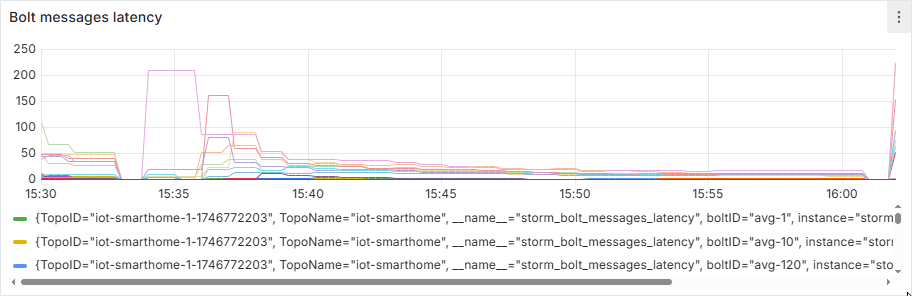
\includegraphics[width=\textwidth]{dq-scale/bolt-messages-latency-01.png}
    \caption{Học tăng cường Q sâu - độ trễ gói tin của các bolt}
    \label{fig:evaluate-bolt-latency}
\end{figure}

Độ trễ của các bolt không có gì quá đặc biệt, chỉ có một khoảng thời gian đạt đỉnh tại khoảng thời gian trước 15:35 nhưng cũng không quá đáng kể, sau khoảng thời gian này, nhờ số lượng supervisor tăng lên 3 nên độ trễ đã giảm dần theo thời gian.

\section{Đánh giá}

\subsection{Đánh giá giữa học tăng cường Q và học tăng cường Q sâu}

Trong hệ thống được sử dụng trong đồ án, các trạng thái của hệ thống và số lượng hành động vẫn đủ nhỏ để có thể ứng dụng hệ thống học tăng cường q. Tuy nhiên, do hạn chế của học tăng cường Q yêu cầu các cặp trạng thái-hành động phải được gặp đủ nhiều và thường xuyên (đủ khám phá) khiến cho chúng khó có thể mở rộng nếu trạng thái hệ thống có thay đổi, chẳng hạn số lượng supervisor tối đa thay đổi, số lượng các hành động thay đổi, v.v. Mặc dù vậy, nhờ sự đơn giản của thuật toán, việc ứng dụng và triển khai rất đơn giản. Hơn nữa, tốc độ hội tụ của học tăng cường Q là được đảm bảo.

Học tăng cường Q sâu là một phiên bản cao cấp hơn của học tăng cường Q mở rộng ra cho các môi trường có trạng thái liên tục thay vì trạng thái rời rạc nơi số lượng trạng thái của môi trường là đủ lớn để có thể lưu thành bảng, đây là một thuật toán cực kỳ phù hợp trong môi trường co/dãn tài nguyên. Tuy nhiên, điểm yếu lớn nhất của phương pháp này đó chính là khả năng hội tụ về giá trị Q tối ưu không được đảm bảo, mặc dù vậy trong các báo cáo thực nghiệm thì học tăng cường Q sâu thường vẫn hội tụ về vùng tiệm cận với giá trị tối ưu \autocite{Zhang2023OnTC}.

Kết hợp hai phương pháp này, ta có được quy trình tối ưu cho việc xây dựng các phương pháp học tăng cường Q sâu cho bài toán học tăng cường như sau: Vận dụng một hệ thống học tăng cường Q đơn giản để tối ưu hàm phần thưởng/hình phạt, sử dụng hàm phần thưởng hình phạt này để huấn luyện các hệ thống học tăng cường Q sâu, sử dụng mô hình được huấn luyện đưa vào tương tác với môi trường và không ngừng tối ưu để thích nghi với sự thay đổi của môi trường.

\subsection{Đánh giá chung}

Một số đánh giá về hệ thống:

\begin{itemize}
    \item \textbf{Khả năng thích ứng cao với môi trường động và không chắc chắn}: Hệ thống đã thể hiện khả năng thích ứng tốt, cho phép tự động điều chỉnh quy mô một cách linh hoạt để đáp ứng hiệu quả các biến động của tải làm việc trong môi trường điện toán đám mây.
    \item \textbf{Tối ưu hóa dựa trên mục tiêu hiệu suất toàn cục và dài hạn}: Hệ thống đã thể hiện khả năng cân bằng giữa tỷ lệ sử dụng bộ nhớ mong muốn, chi phí vận hành cùng dựa trên nhiều trạng thái chỉ số của môi trường.
    \item \textbf{Khả năng tự động hóa, giảm thiểu chi phí quản lý}: Hệ thống tự động co/dãn mà không cần can thiệp thủ công giúp giảm thiểu chi phí quản lý, các lỗi thao tác phát sinh và tăng tốc độ triển khai, giải phóng nhân lực để sử dụng cho các tác vụ phức tạp hơn.
\end{itemize}

\begin{figure}[htbp]
    \centering
    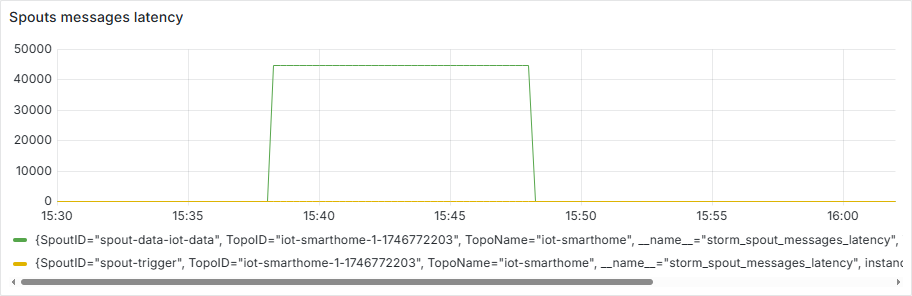
\includegraphics[width=\textwidth]{dq-scale/spout-messages-latency-01.png}
    \caption{Độ trễ của các spout}
    \label{fig:evaluate-dq-spout-latency}
\end{figure}

Ngoài các ưu điểm trên, vẫn còn các yếu điểm cần được khắc phục cùng với các nhược điểm của hệ thống và mô hình học tăng cường như sau:

\begin{itemize}
    \item \textbf{Cải thiện hệ thống SmartHome}: Cần tăng luồng xử lý cho các thành phần, điển hình là các spout - thành phần cung cấp dữ liệu đầu vào của hệ thống hiện tại đang chỉ sử dụng duy nhất 1 parallelism sẽ gây ra nghẽn cho hệ thống bất kể hiệu năng đang được sử dụng của spout. Điều này thể hiện rõ qua hình \ref{fig:evaluate-dq-spout-latency} và hình \ref{fig:evaluate-dq-memory-usage} khi hiệu năng của các supervisor vẫn trong ngưỡng cho phép nhưng độ trễ tăng đột biến vượt quá mức kiểm soát.
    \item \textbf{Hạn chế tài nguyên huấn luyện và đánh giá}: Thời gian giữa các lần co/dãn trong luận án này khá bé khiến cho độ ổn định của topology không cao đồng thời cũng không phù hợp với hệ thống thật khi thời gian co/dãn sẽ được kéo dài hơn. Các máy ảo được sử dụng trên GCP thường xuyên có cấu hình kém, thường xuyên bị chết trong quá trình đánh giá, gây kết quả sai lệch.
    \item \textbf{Thao tác co/dãn đơn giản}: các thao tác co/dãn còn đơn giản, chưa thực sự phù hợp với thực tế khi số lượng các supervisor tăng lên. Khi đó, thời gian cần thiết để đáp ứng tải với chiến thuật co/dãn một supervisor sẽ khá lâu.
    \item \textbf{Thách thức mô hình hóa bài toán thực tế}: độ phức tạp trong việc định nghĩa chính xác bài toán học tăng cường (trạng thái, hành động, phần thưởng), khiến cho việc tối ưu và đánh giá gặp không ít trở ngại.
    \item \textbf{Chi phí huấn luyện}: hai yêu cầu trong đó yêu cầu tương tác với môi trường (đặc trưng của học tăng cường) và yêu cầu lượng dữ liệu đầu vào lớn (đặc trưng của các thuật toán học máy) khiến cho chi phí và thời gian huấn luyện cao so với các thuật toán học máy có giám sát truyền thống.
    \item \textbf{Khác biệt môi trường}: Luôn có khoảng cách giữa môi trường mô phỏng và thực tế đặt ra yêu cầu về kỹ thuật cao, các kỹ sư phát triển cần nắm rõ hệ thống cũng như bao quát các vấn đề có thể phát sinh trong tương lai.
\end{itemize}